% Options for packages loaded elsewhere
\PassOptionsToPackage{unicode}{hyperref}
\PassOptionsToPackage{hyphens}{url}
%
\documentclass[
  ignorenonframetext,
]{beamer}
\usepackage{pgfpages}
\setbeamertemplate{caption}[numbered]
\setbeamertemplate{caption label separator}{: }
\setbeamercolor{caption name}{fg=normal text.fg}
\beamertemplatenavigationsymbolsempty
% Prevent slide breaks in the middle of a paragraph
\widowpenalties 1 10000
\raggedbottom
\setbeamertemplate{part page}{
  \centering
  \begin{beamercolorbox}[sep=16pt,center]{part title}
    \usebeamerfont{part title}\insertpart\par
  \end{beamercolorbox}
}
\setbeamertemplate{section page}{
  \centering
  \begin{beamercolorbox}[sep=12pt,center]{part title}
    \usebeamerfont{section title}\insertsection\par
  \end{beamercolorbox}
}
\setbeamertemplate{subsection page}{
  \centering
  \begin{beamercolorbox}[sep=8pt,center]{part title}
    \usebeamerfont{subsection title}\insertsubsection\par
  \end{beamercolorbox}
}
\AtBeginPart{
  \frame{\partpage}
}
\AtBeginSection{
  \ifbibliography
  \else
    \frame{\sectionpage}
  \fi
}
\AtBeginSubsection{
  \frame{\subsectionpage}
}
\usepackage{amsmath,amssymb}
\usepackage{lmodern}
\usepackage{ifxetex,ifluatex}
\ifnum 0\ifxetex 1\fi\ifluatex 1\fi=0 % if pdftex
  \usepackage[T1]{fontenc}
  \usepackage[utf8]{inputenc}
  \usepackage{textcomp} % provide euro and other symbols
\else % if luatex or xetex
  \usepackage{unicode-math}
  \defaultfontfeatures{Scale=MatchLowercase}
  \defaultfontfeatures[\rmfamily]{Ligatures=TeX,Scale=1}
\fi
% Use upquote if available, for straight quotes in verbatim environments
\IfFileExists{upquote.sty}{\usepackage{upquote}}{}
\IfFileExists{microtype.sty}{% use microtype if available
  \usepackage[]{microtype}
  \UseMicrotypeSet[protrusion]{basicmath} % disable protrusion for tt fonts
}{}
\makeatletter
\@ifundefined{KOMAClassName}{% if non-KOMA class
  \IfFileExists{parskip.sty}{%
    \usepackage{parskip}
  }{% else
    \setlength{\parindent}{0pt}
    \setlength{\parskip}{6pt plus 2pt minus 1pt}}
}{% if KOMA class
  \KOMAoptions{parskip=half}}
\makeatother
\usepackage{xcolor}
\IfFileExists{xurl.sty}{\usepackage{xurl}}{} % add URL line breaks if available
\IfFileExists{bookmark.sty}{\usepackage{bookmark}}{\usepackage{hyperref}}
\hypersetup{
  pdftitle={ESA-listed rockfishes working group meeting},
  pdfauthor={Markus Min},
  hidelinks,
  pdfcreator={LaTeX via pandoc}}
\urlstyle{same} % disable monospaced font for URLs
\newif\ifbibliography
\usepackage{graphicx}
\makeatletter
\def\maxwidth{\ifdim\Gin@nat@width>\linewidth\linewidth\else\Gin@nat@width\fi}
\def\maxheight{\ifdim\Gin@nat@height>\textheight\textheight\else\Gin@nat@height\fi}
\makeatother
% Scale images if necessary, so that they will not overflow the page
% margins by default, and it is still possible to overwrite the defaults
% using explicit options in \includegraphics[width, height, ...]{}
\setkeys{Gin}{width=\maxwidth,height=\maxheight,keepaspectratio}
% Set default figure placement to htbp
\makeatletter
\def\fps@figure{htbp}
\makeatother
\setlength{\emergencystretch}{3em} % prevent overfull lines
\providecommand{\tightlist}{%
  \setlength{\itemsep}{0pt}\setlength{\parskip}{0pt}}
\setcounter{secnumdepth}{-\maxdimen} % remove section numbering
\ifluatex
  \usepackage{selnolig}  % disable illegal ligatures
\fi

\title{ESA-listed rockfishes working group meeting}
\author{Markus Min}
\date{5/25/2021}

\begin{document}
\frame{\titlepage}

\begin{frame}{ROV surveys}
\protect\hypertarget{rov-surveys}{}
\begin{itemize}
\tightlist
\item
  2008 San Juan Islands
\item
  2010 San Juan Islands
\item
  2015-16 Puget Sound
\item
  2018 San Juan Islands
\item
  2018 Vector Survey (Strait of Georgia)
\item
  2018 Gulf Islands Survey
\end{itemize}
\end{frame}

\begin{frame}{Uses of ROV data for 5-year review}
\protect\hypertarget{uses-of-rov-data-for-5-year-review}{}
\begin{itemize}
\tightlist
\item
  As an index of abundance for assessment model

  \begin{itemize}
  \tightlist
  \item
    Single time point of absolute abundance across entire DPS (as in the
    case of Hood Canal)
  \item
    Time series of abundances from the same geographic area (as in the
    case of the San Juan Islands)
  \end{itemize}
\item
  As an index of abundance to compare with reference points from the
  assessment model
\item
  To stress how repeated ROV surveys would allow us to track population
  dynamics without needing to do a formal assessment
\end{itemize}
\end{frame}

\begin{frame}{What is the selectivity of ROV surveys? \textbar{} Key to
contextualizing abundance estimates}
\protect\hypertarget{what-is-the-selectivity-of-rov-surveys-key-to-contextualizing-abundance-estimates}{}
\begin{itemize}
\tightlist
\item
  What types of individuals are seen by the ROV?
\item
  What proportion of these individuals are seen by the ROV?
\end{itemize}

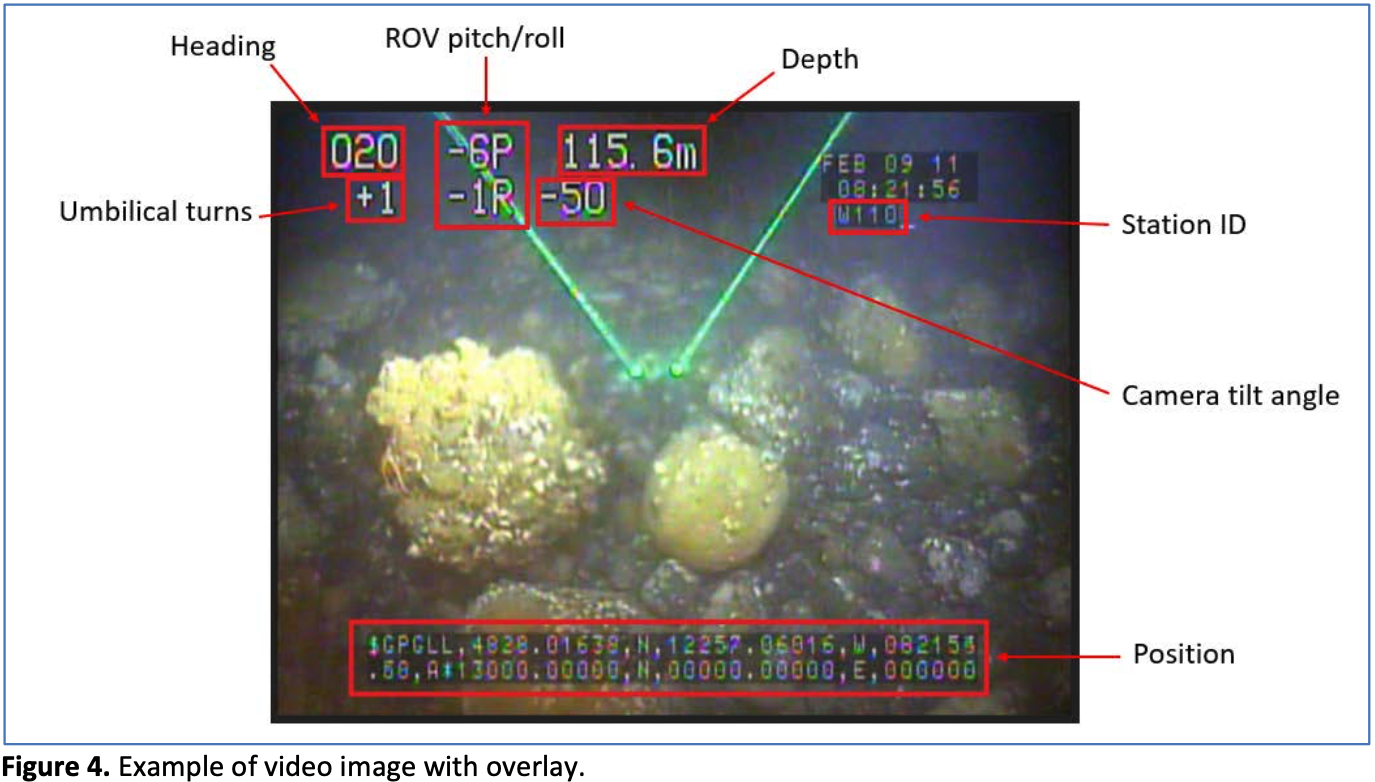
\includegraphics[width=0.8\textwidth,height=\textheight]{ROV_example_video.png}
\end{frame}

\begin{frame}{Calculating abundance}
\protect\hypertarget{calculating-abundance}{}
The mean stratum density (\(\overline{D_s}\)) for a given taxon was the
the sum of the individual transect densities divided by the number of
transects (\(N_s\)):

\[
\overline{D_s} = \frac{\sum\limits_{i=1}^N D_i} {N_s}
\] Total abundance (\(P\)) in numbers of individuals was the product of
the stratum surface area (\(SA_s\)) and the mean taxon density
(\(\overline{D_s}\)), with variance calculated as the product of surface
area and the variance of mean stratum density:

\[
P_s = SA_s\overline{D_s};Var(P_s) = SA_sVar(\overline{D_s})
\]
\end{frame}

\begin{frame}{ROV abundance results}
\protect\hypertarget{rov-abundance-results}{}
\begin{table}[H]
\centering\begingroup\fontsize{16}{18}\selectfont

\begin{tabular}{l|l|l|l|r|r}
\hline
survey & area & year & species & abundance & CV\\
\hline
2008 San Juan Islands & San Juan Islands & 2008 & Yelloweye Rockfish & 47,407 & 25\\
\hline
2010 San Juan Islands & San Juan Islands & 2010 & Yelloweye Rockfish & 114,494 & 33\\
\hline
2015-16 Puget Sound & Puget Sound Proper (excluding Hood Canal) & 2015, 2016 & Yelloweye Rockfish & 6,285 & 29\\
\hline
2015-16 Puget Sound & Hood Canal & 2015, 2016 & Yelloweye Rockfish & 14,699 & 23\\
\hline
2018 San Juan Islands & San Juan Islands & 2018 & Yelloweye Rockfish & 17,121 & 37\\
\hline
2018 Gulf Islands - High Stratum & Gulf Islands (Inside) & 2018 & Yelloweye Rockfish & 83,783 & 34\\
\hline
2018 Gulf Islands - Medium Stratum & Gulf Islands (Inside) & 2018 & Yelloweye Rockfish & 58,887 & 72\\
\hline
2018 Vector & Strait of Georgia (CA) & 2018 & Yelloweye Rockfish & 1,613,716 & 14\\
\hline
\end{tabular}
\endgroup{}
\end{table}
\end{frame}

\begin{frame}{2015-16 Puget Sound Survey}
\protect\hypertarget{puget-sound-survey}{}
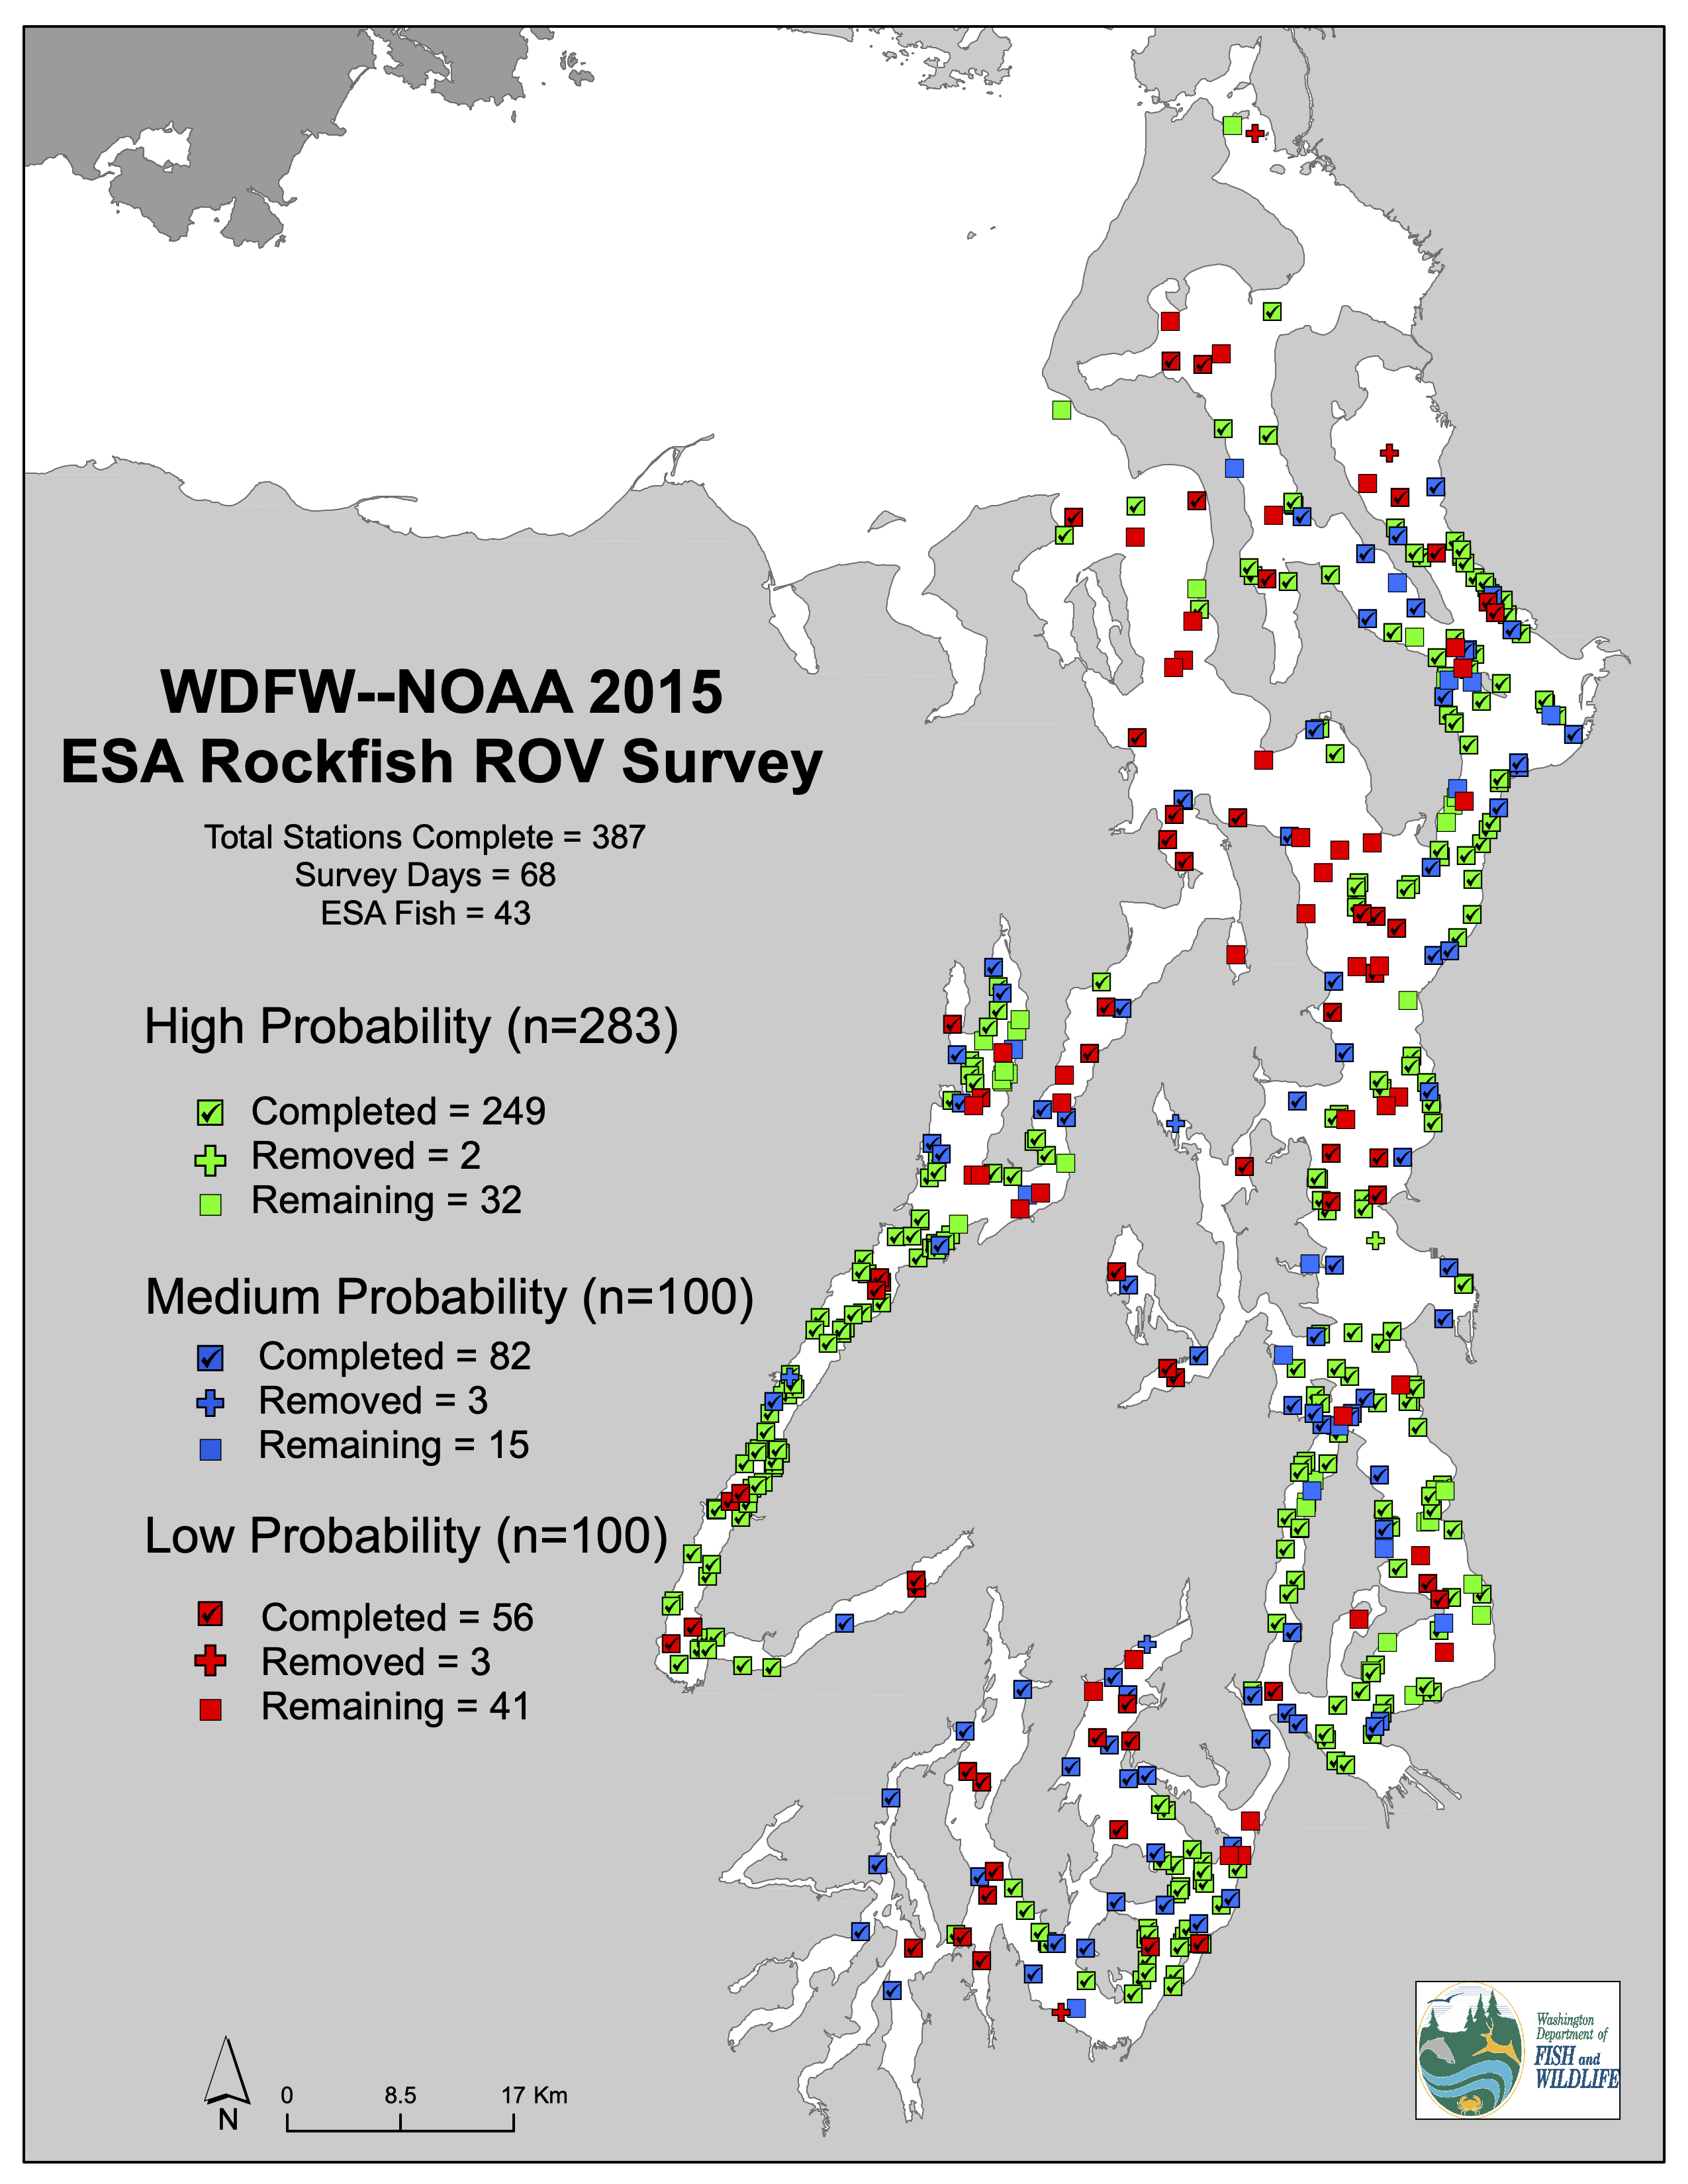
\includegraphics[width=1\textwidth,height=\textheight]{2015_PS_map.png}

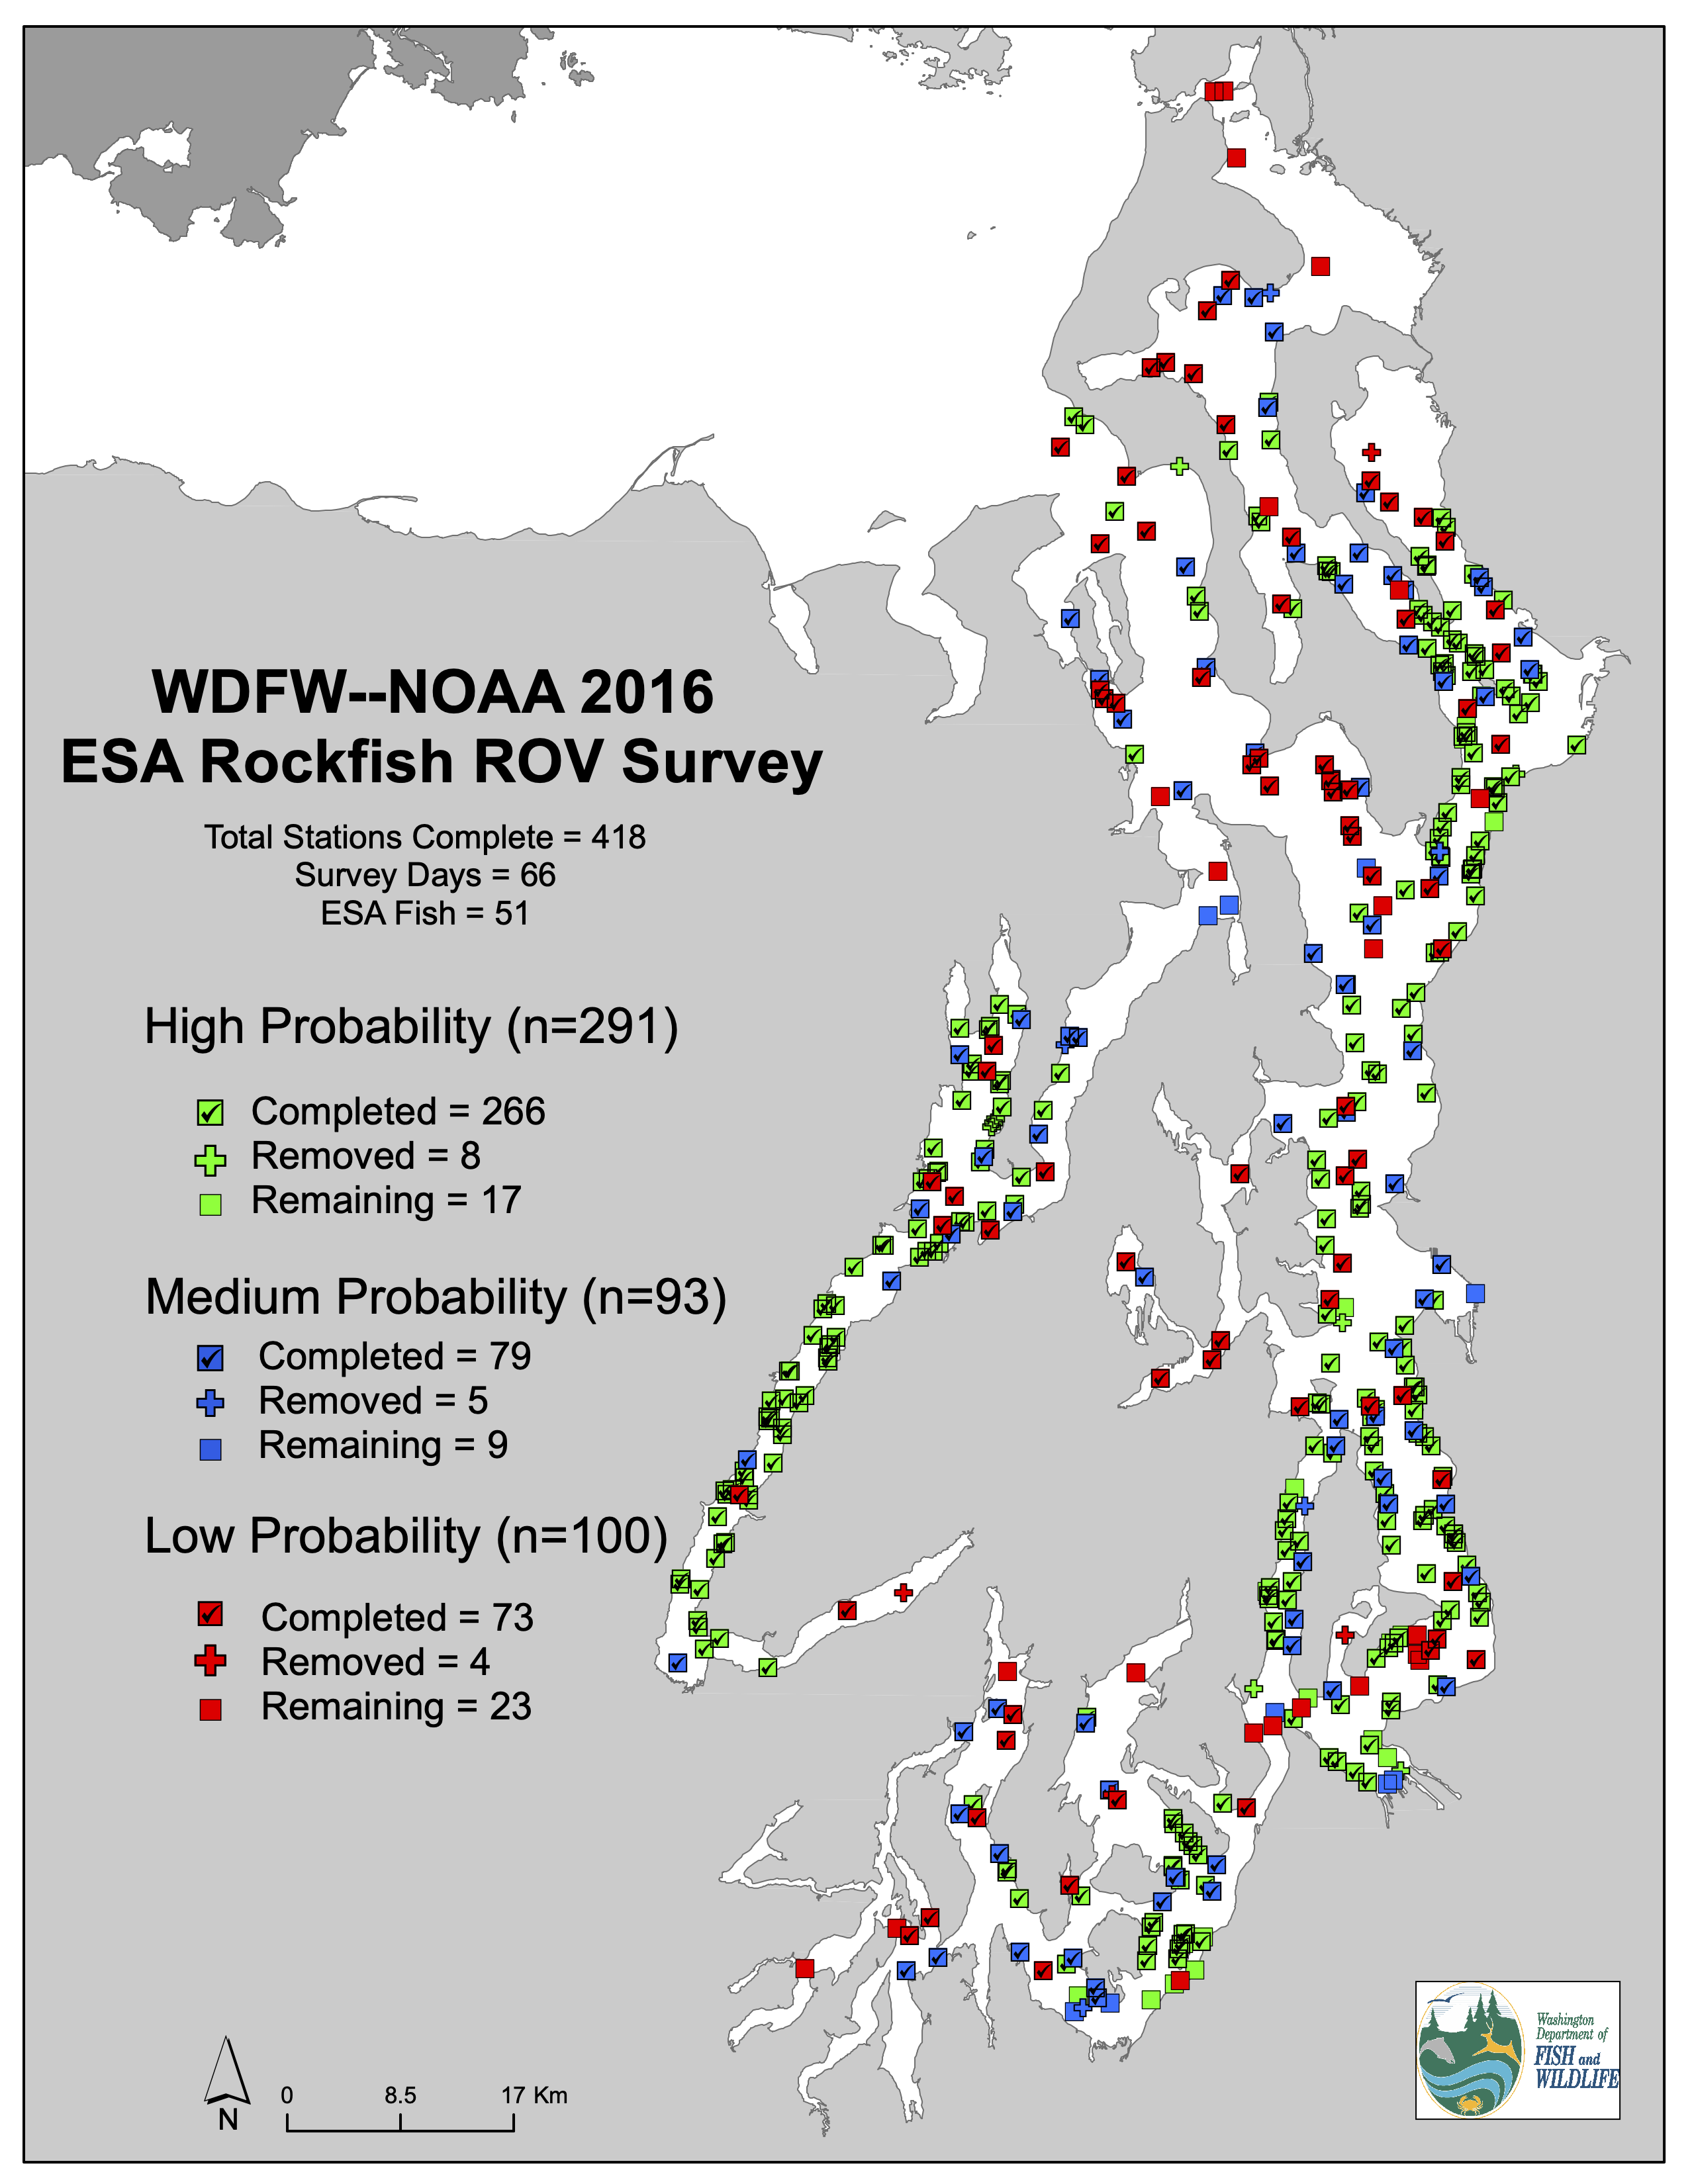
\includegraphics[width=1\textwidth,height=\textheight]{2016_PS_map.png}
\end{frame}

\begin{frame}{2015-16 Puget Sound}
\protect\hypertarget{puget-sound}{}
\begin{itemize}
\tightlist
\item
  Maximum entropy model used to determine habitat suitability, based on
  combination of previous occurrences of yelloweye and habitat
  characteristics
\end{itemize}

\begin{block}{non-Hood Canal}
\protect\hypertarget{non-hood-canal}{}
\begin{itemize}
\tightlist
\item
  Survey strata: ``High'', ``Medium'', ``Low''

  \begin{itemize}
  \tightlist
  \item
    High stratum

    \begin{itemize}
    \tightlist
    \item
      363 transects
    \item
      9,288 hectares
    \item
      25 yelloweye
    \end{itemize}
  \item
    Medium + Low strata

    \begin{itemize}
    \tightlist
    \item
      244 transects
    \item
      1,058,427 hectares
    \item
      0 yelloweye
    \end{itemize}
  \end{itemize}
\item
  Population estimate: 6,285 (CV = 29.5\%)
\end{itemize}
\end{block}

\begin{block}{Hood Canal}
\protect\hypertarget{hood-canal}{}
\begin{itemize}
\tightlist
\item
  Survey strata: ``High'', ``Medium'', ``Low''

  \begin{itemize}
  \tightlist
  \item
    High stratum

    \begin{itemize}
    \tightlist
    \item
      152 transects
    \item
      4,486 hectares
    \item
      25 yelloweye
    \end{itemize}
  \item
    Medium + Low strata

    \begin{itemize}
    \tightlist
    \item
      46 transects
    \item
      120,637 hectares
    \item
      0 yelloweye
    \end{itemize}
  \end{itemize}
\item
  Population estimate: 14,699 (CV = 22.9\%)
\end{itemize}
\end{block}
\end{frame}

\begin{frame}{2008 SJI ROV survey}
\protect\hypertarget{sji-rov-survey}{}
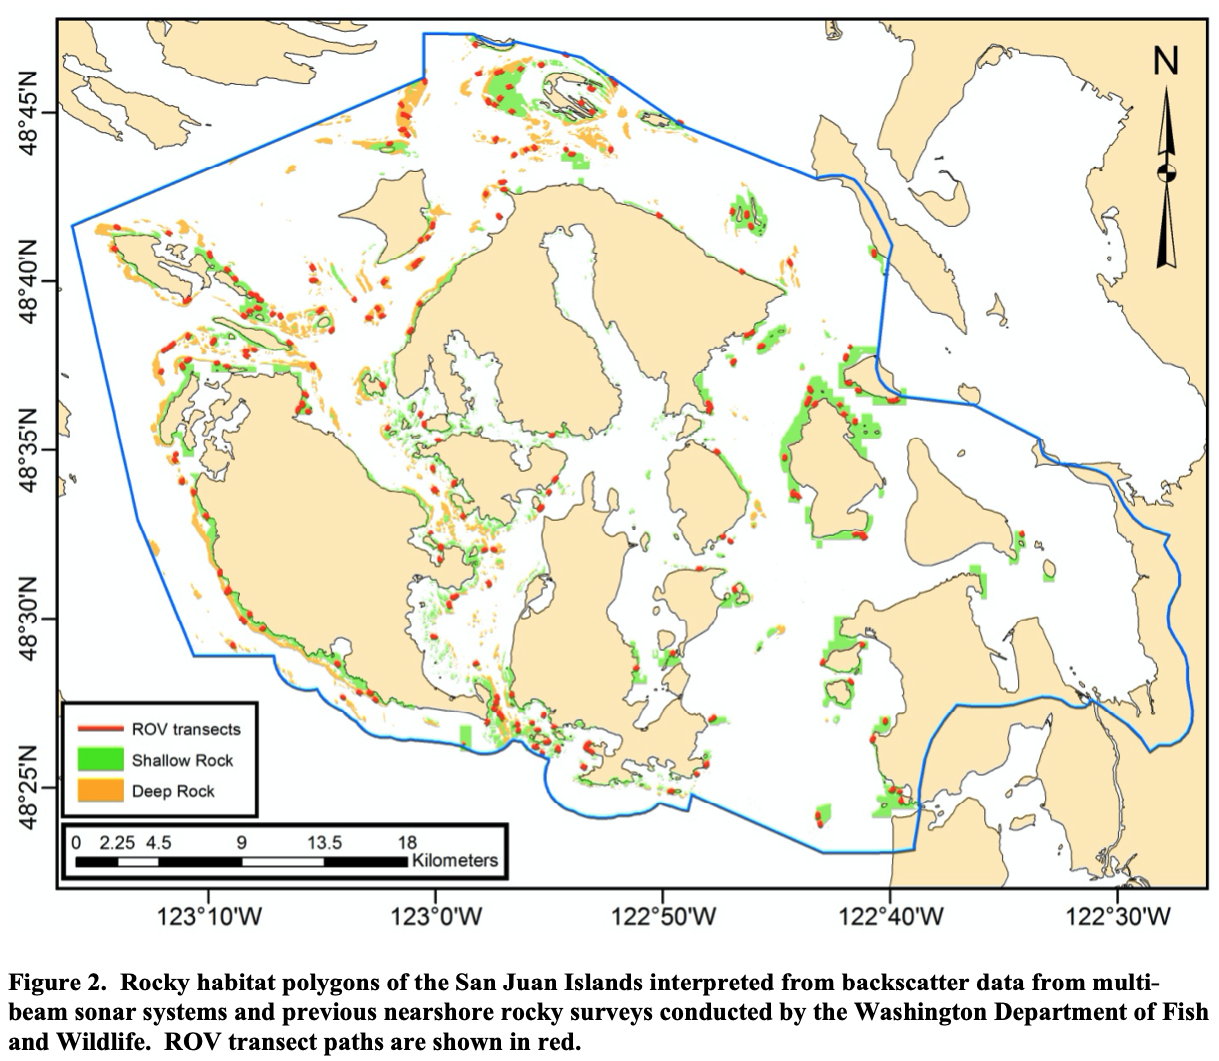
\includegraphics[width=1\textwidth,height=\textheight]{2008_SJI_map.png}

\begin{itemize}
\tightlist
\item
  Rocky habitat identified using MBES (multibeam echosounder)
\item
  Survey strata: ``Shallow rock'' and ``Deep rock''

  \begin{itemize}
  \tightlist
  \item
    Shallow rock

    \begin{itemize}
    \tightlist
    \item
      136 transects
    \item
      7,860 hectares
    \item
      1 yelloweye
    \end{itemize}
  \item
    Deep rock

    \begin{itemize}
    \tightlist
    \item
      71 transects
    \item
      4,150 hectares
    \item
      38 yelloweye
    \end{itemize}
  \end{itemize}
\item
  Population estimate: 47,407 (CV = 24.8\%)
\end{itemize}
\end{frame}

\begin{frame}{2010 SJI ROV survey}
\protect\hypertarget{sji-rov-survey-1}{}
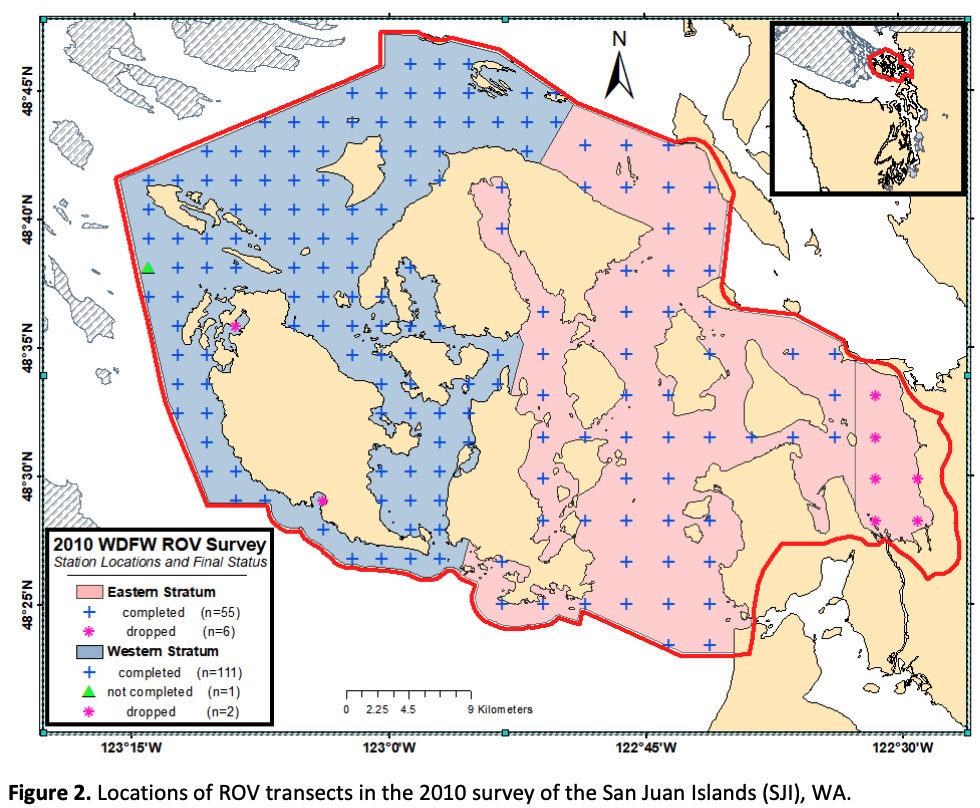
\includegraphics[width=1\textwidth,height=\textheight]{2010_SJI_map.png}

\begin{itemize}
\tightlist
\item
  Systematic grid used to determine transect locations; higher density
  of transects in Western SJI because of previous observations
\item
  Survey strata: ``Eastern SJI'' and ``Western SJI''

  \begin{itemize}
  \tightlist
  \item
    Eastern SJI

    \begin{itemize}
    \tightlist
    \item
      55 transects
    \item
      50,850 hectares
    \item
      0 yelloweye
    \end{itemize}
  \item
    Western SJI

    \begin{itemize}
    \tightlist
    \item
      111 transects
    \item
      53,164 hectares
    \item
      16 yelloweye
    \end{itemize}
  \end{itemize}
\item
  Population estimate: 114,494 (CV = 44.0\%)
\end{itemize}
\end{frame}

\begin{frame}{2018 SJI ROV survey}
\protect\hypertarget{sji-rov-survey-2}{}
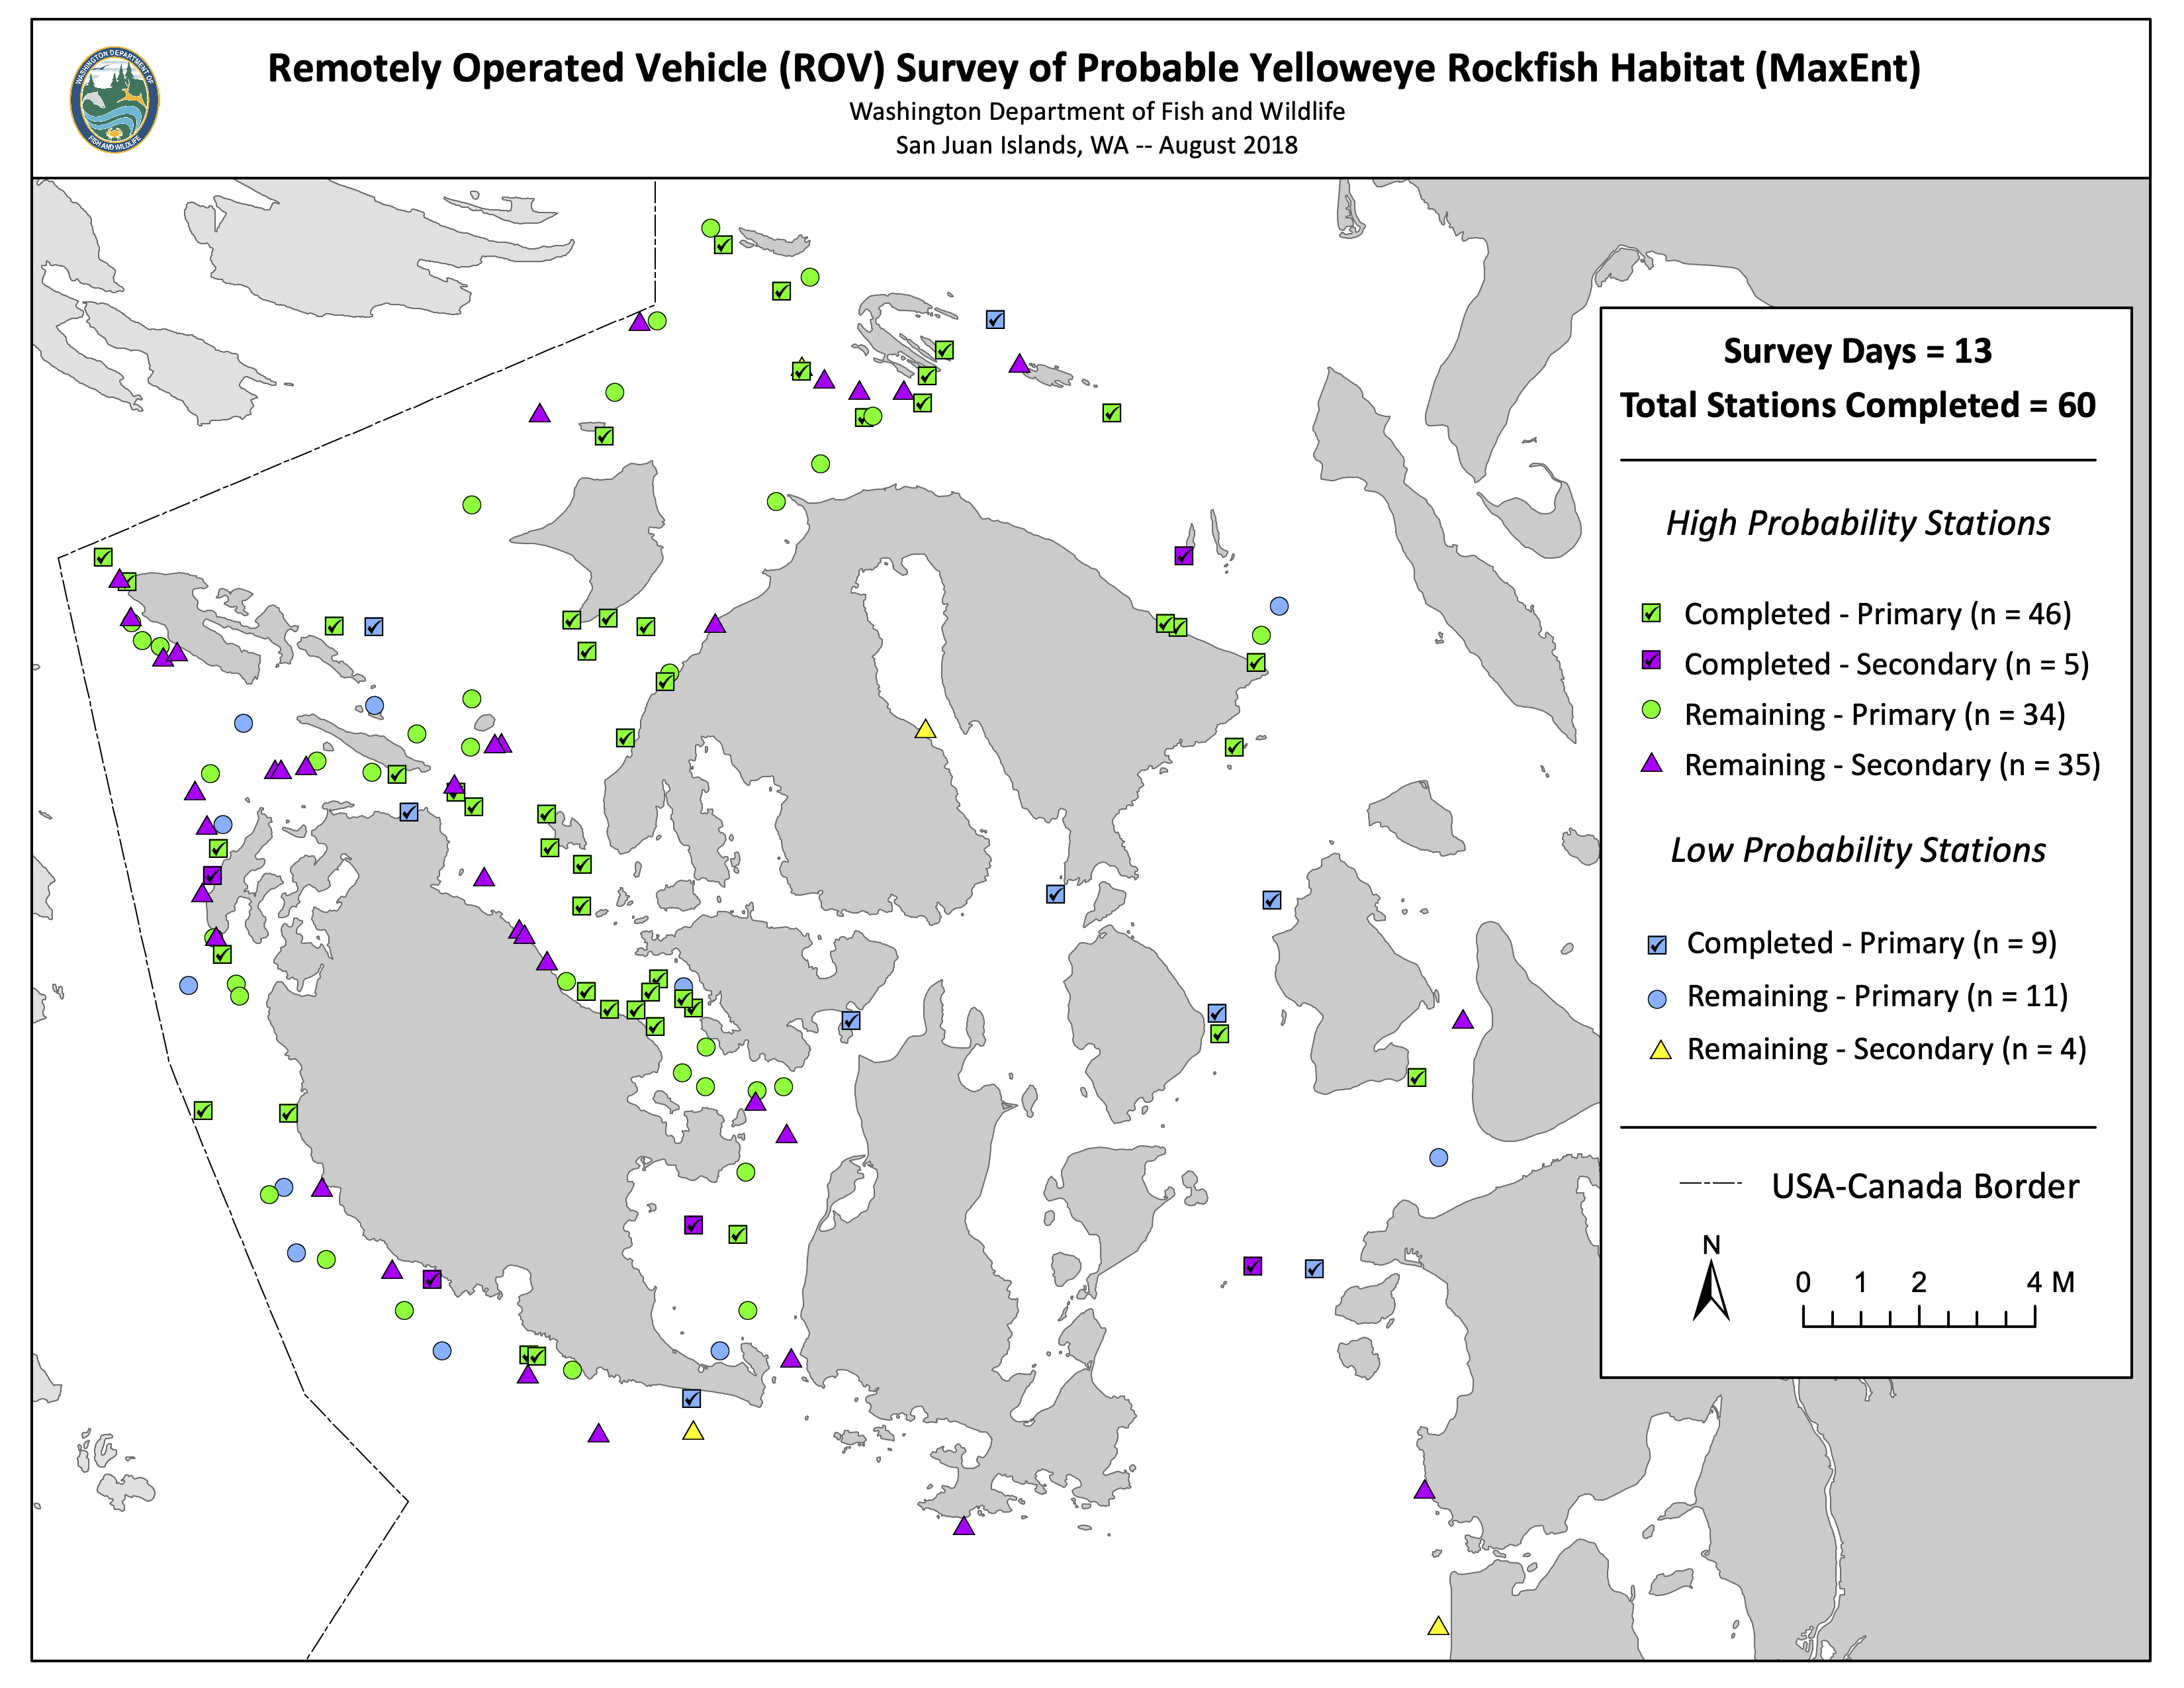
\includegraphics[width=1\textwidth,height=\textheight]{2018_SJI_map.png}

Note: Still waiting on data for two transects for this survey.

\begin{itemize}
\tightlist
\item
  Maximum entropy model used to determine habitat suitability, based on
  combination of previous occurrences of yelloweye and habitat
  characteristics
\item
  Survey strata: ``High'' and ``Low''

  \begin{itemize}
  \tightlist
  \item
    High stratum

    \begin{itemize}
    \tightlist
    \item
      51 transects
    \item
      6,036 hectares
    \item
      14 yelloweye
    \end{itemize}
  \item
    Low stratum

    \begin{itemize}
    \tightlist
    \item
      9 transects
    \item
      102,115 hectares
    \item
      0 yelloweye
    \end{itemize}
  \end{itemize}
\item
  Population estimate: 17,121 (CV = 37.4\%)
\end{itemize}
\end{frame}

\begin{frame}{2018 Gulf Islands survey}
\protect\hypertarget{gulf-islands-survey}{}
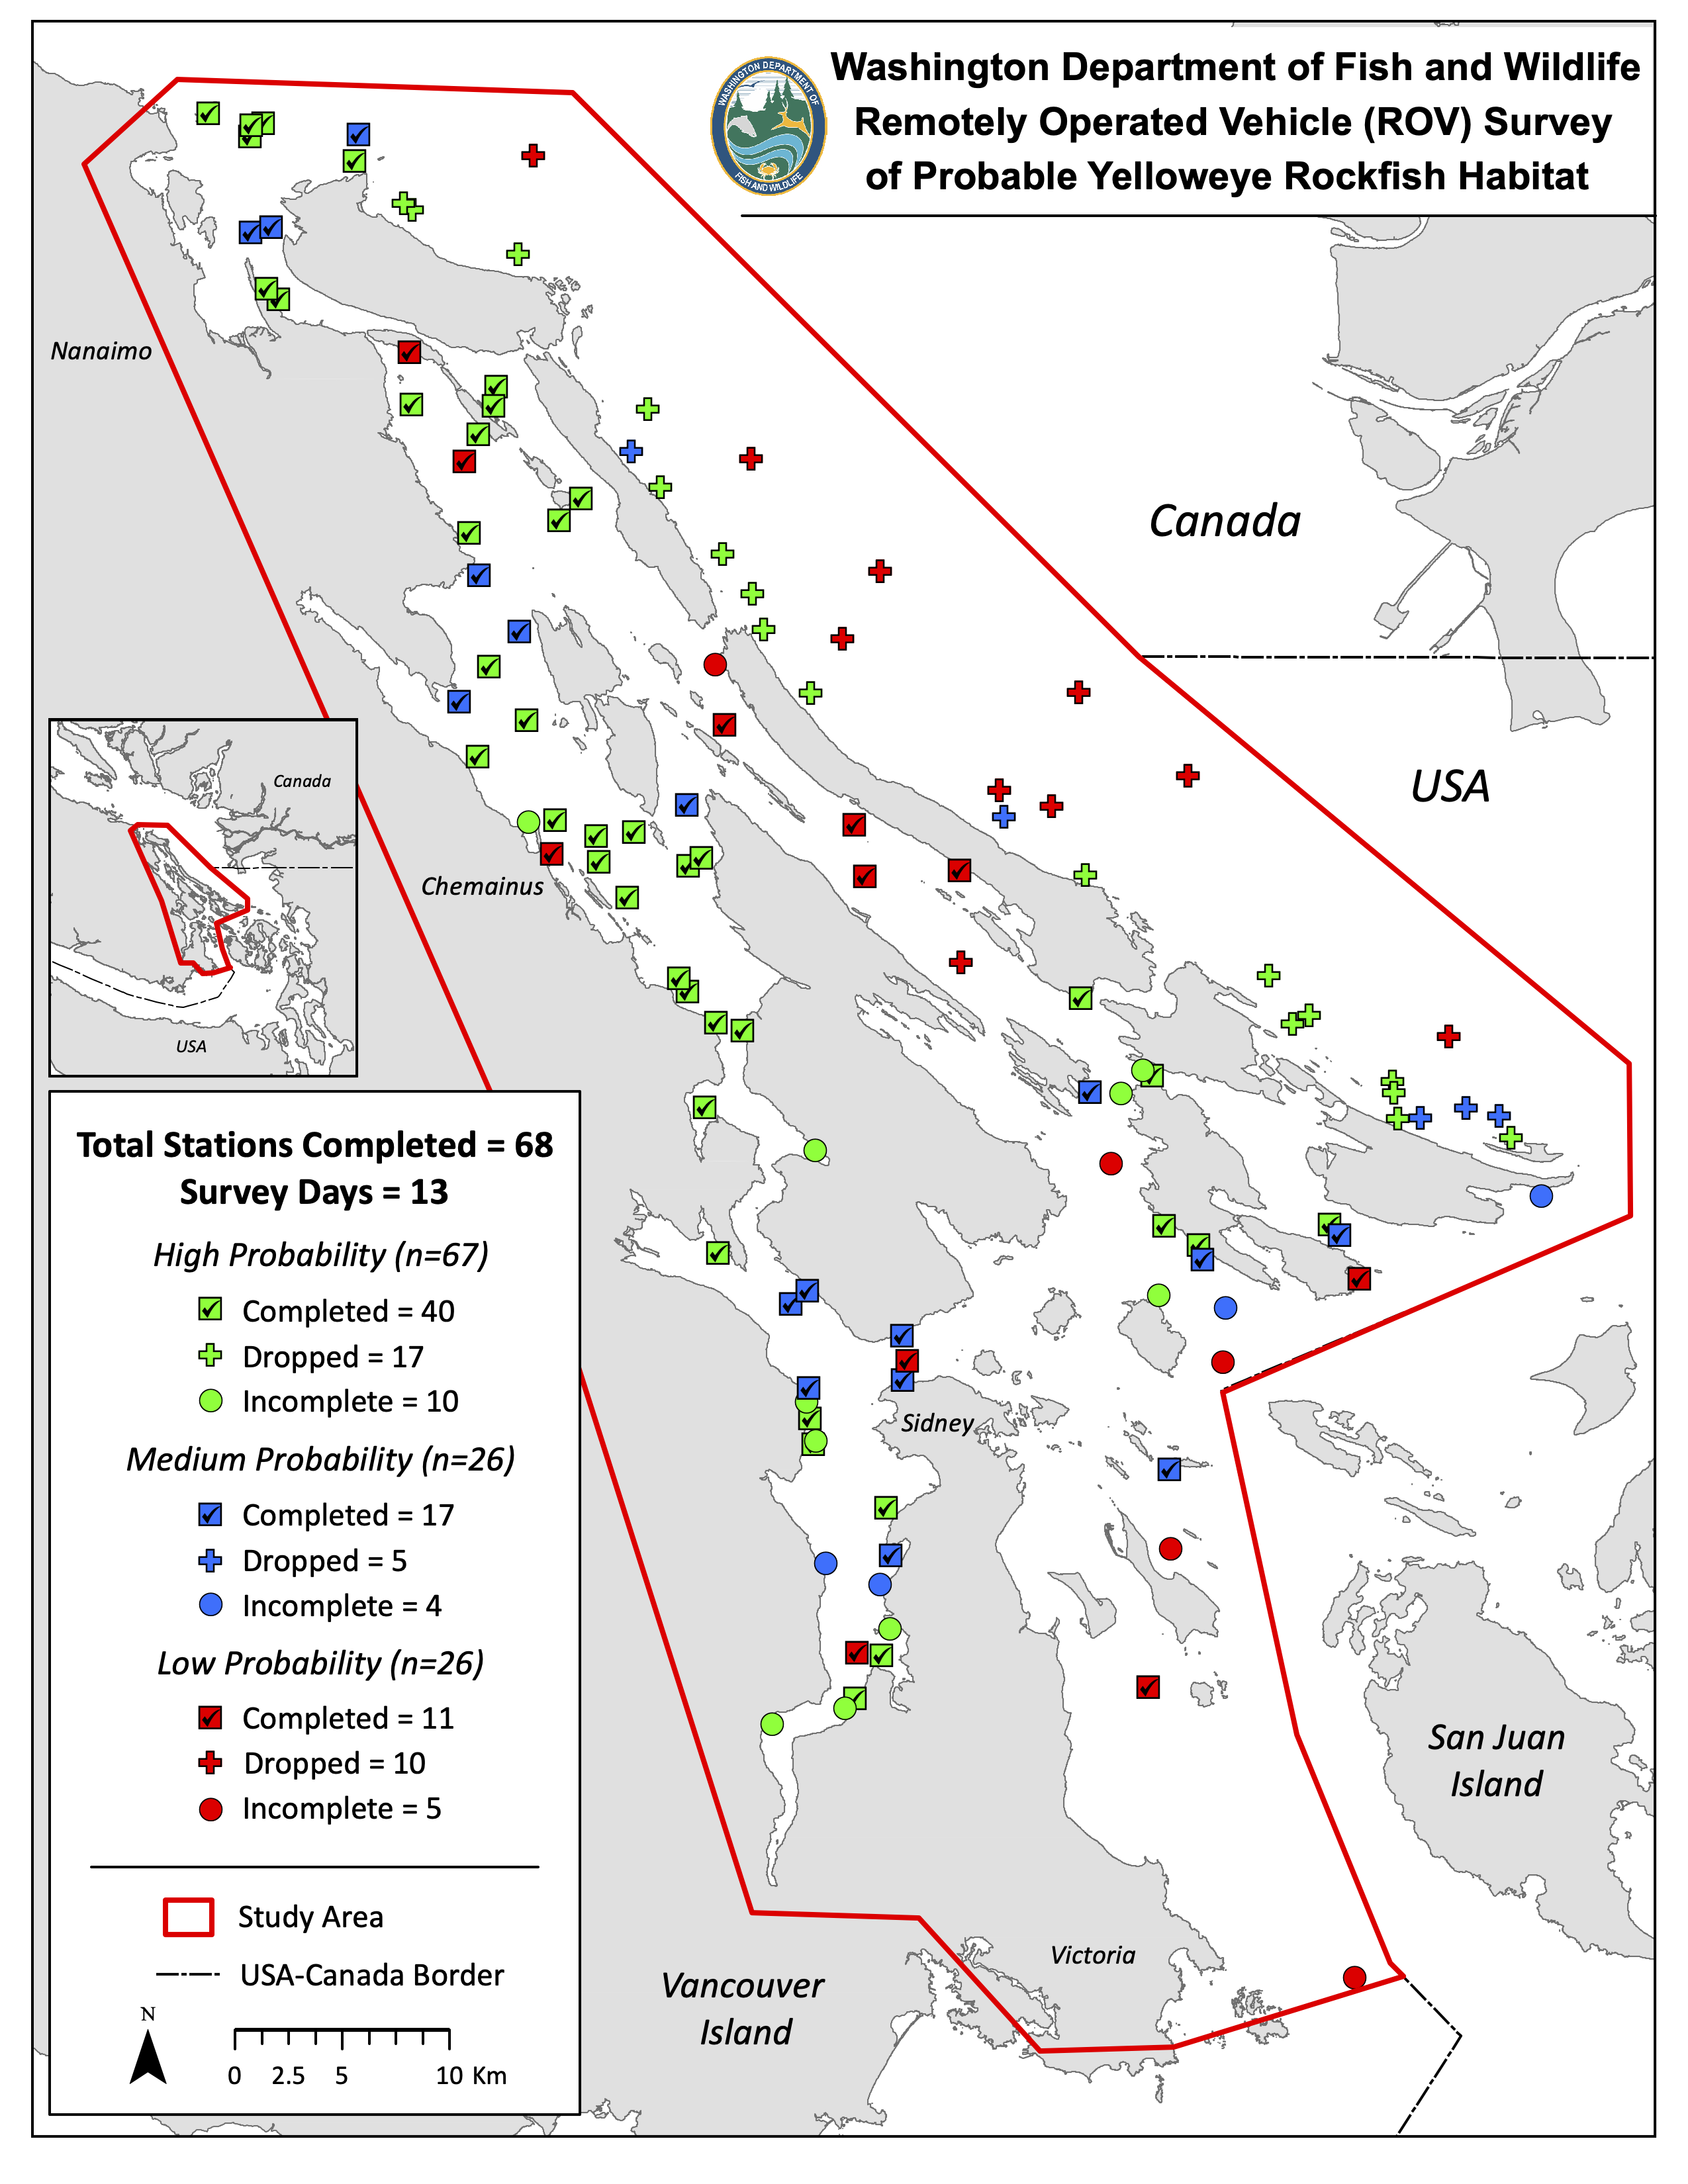
\includegraphics[width=1\textwidth,height=\textheight]{2018_GI_map.png}

\begin{itemize}
\tightlist
\item
  Maximum entropy (maxent) model
\item
  Survey strata: ``High'', ``Medium'', ``Low''

  \begin{itemize}
  \tightlist
  \item
    High stratum

    \begin{itemize}
    \tightlist
    \item
      40 transects
    \item
      6,070 hectares
    \item
      49 yelloweye
    \end{itemize}
  \item
    Medium stratum

    \begin{itemize}
    \tightlist
    \item
      17 transects
    \item
      21,462 hectares
    \item
      4 yelloweye
    \end{itemize}
  \item
    Low stratum

    \begin{itemize}
    \tightlist
    \item
      11 transects
    \item
      76,206 hectares
    \item
      0 yelloweye
    \end{itemize}
  \end{itemize}
\item
  Population estimates:

  \begin{itemize}
  \tightlist
  \item
    High stratum: 83,783 (CV = 34.3\%)
  \item
    Medium stratum: 58,887 (CV = 71.8\%)
  \end{itemize}
\end{itemize}
\end{frame}

\begin{frame}{2018 Vector survey}
\protect\hypertarget{vector-survey}{}
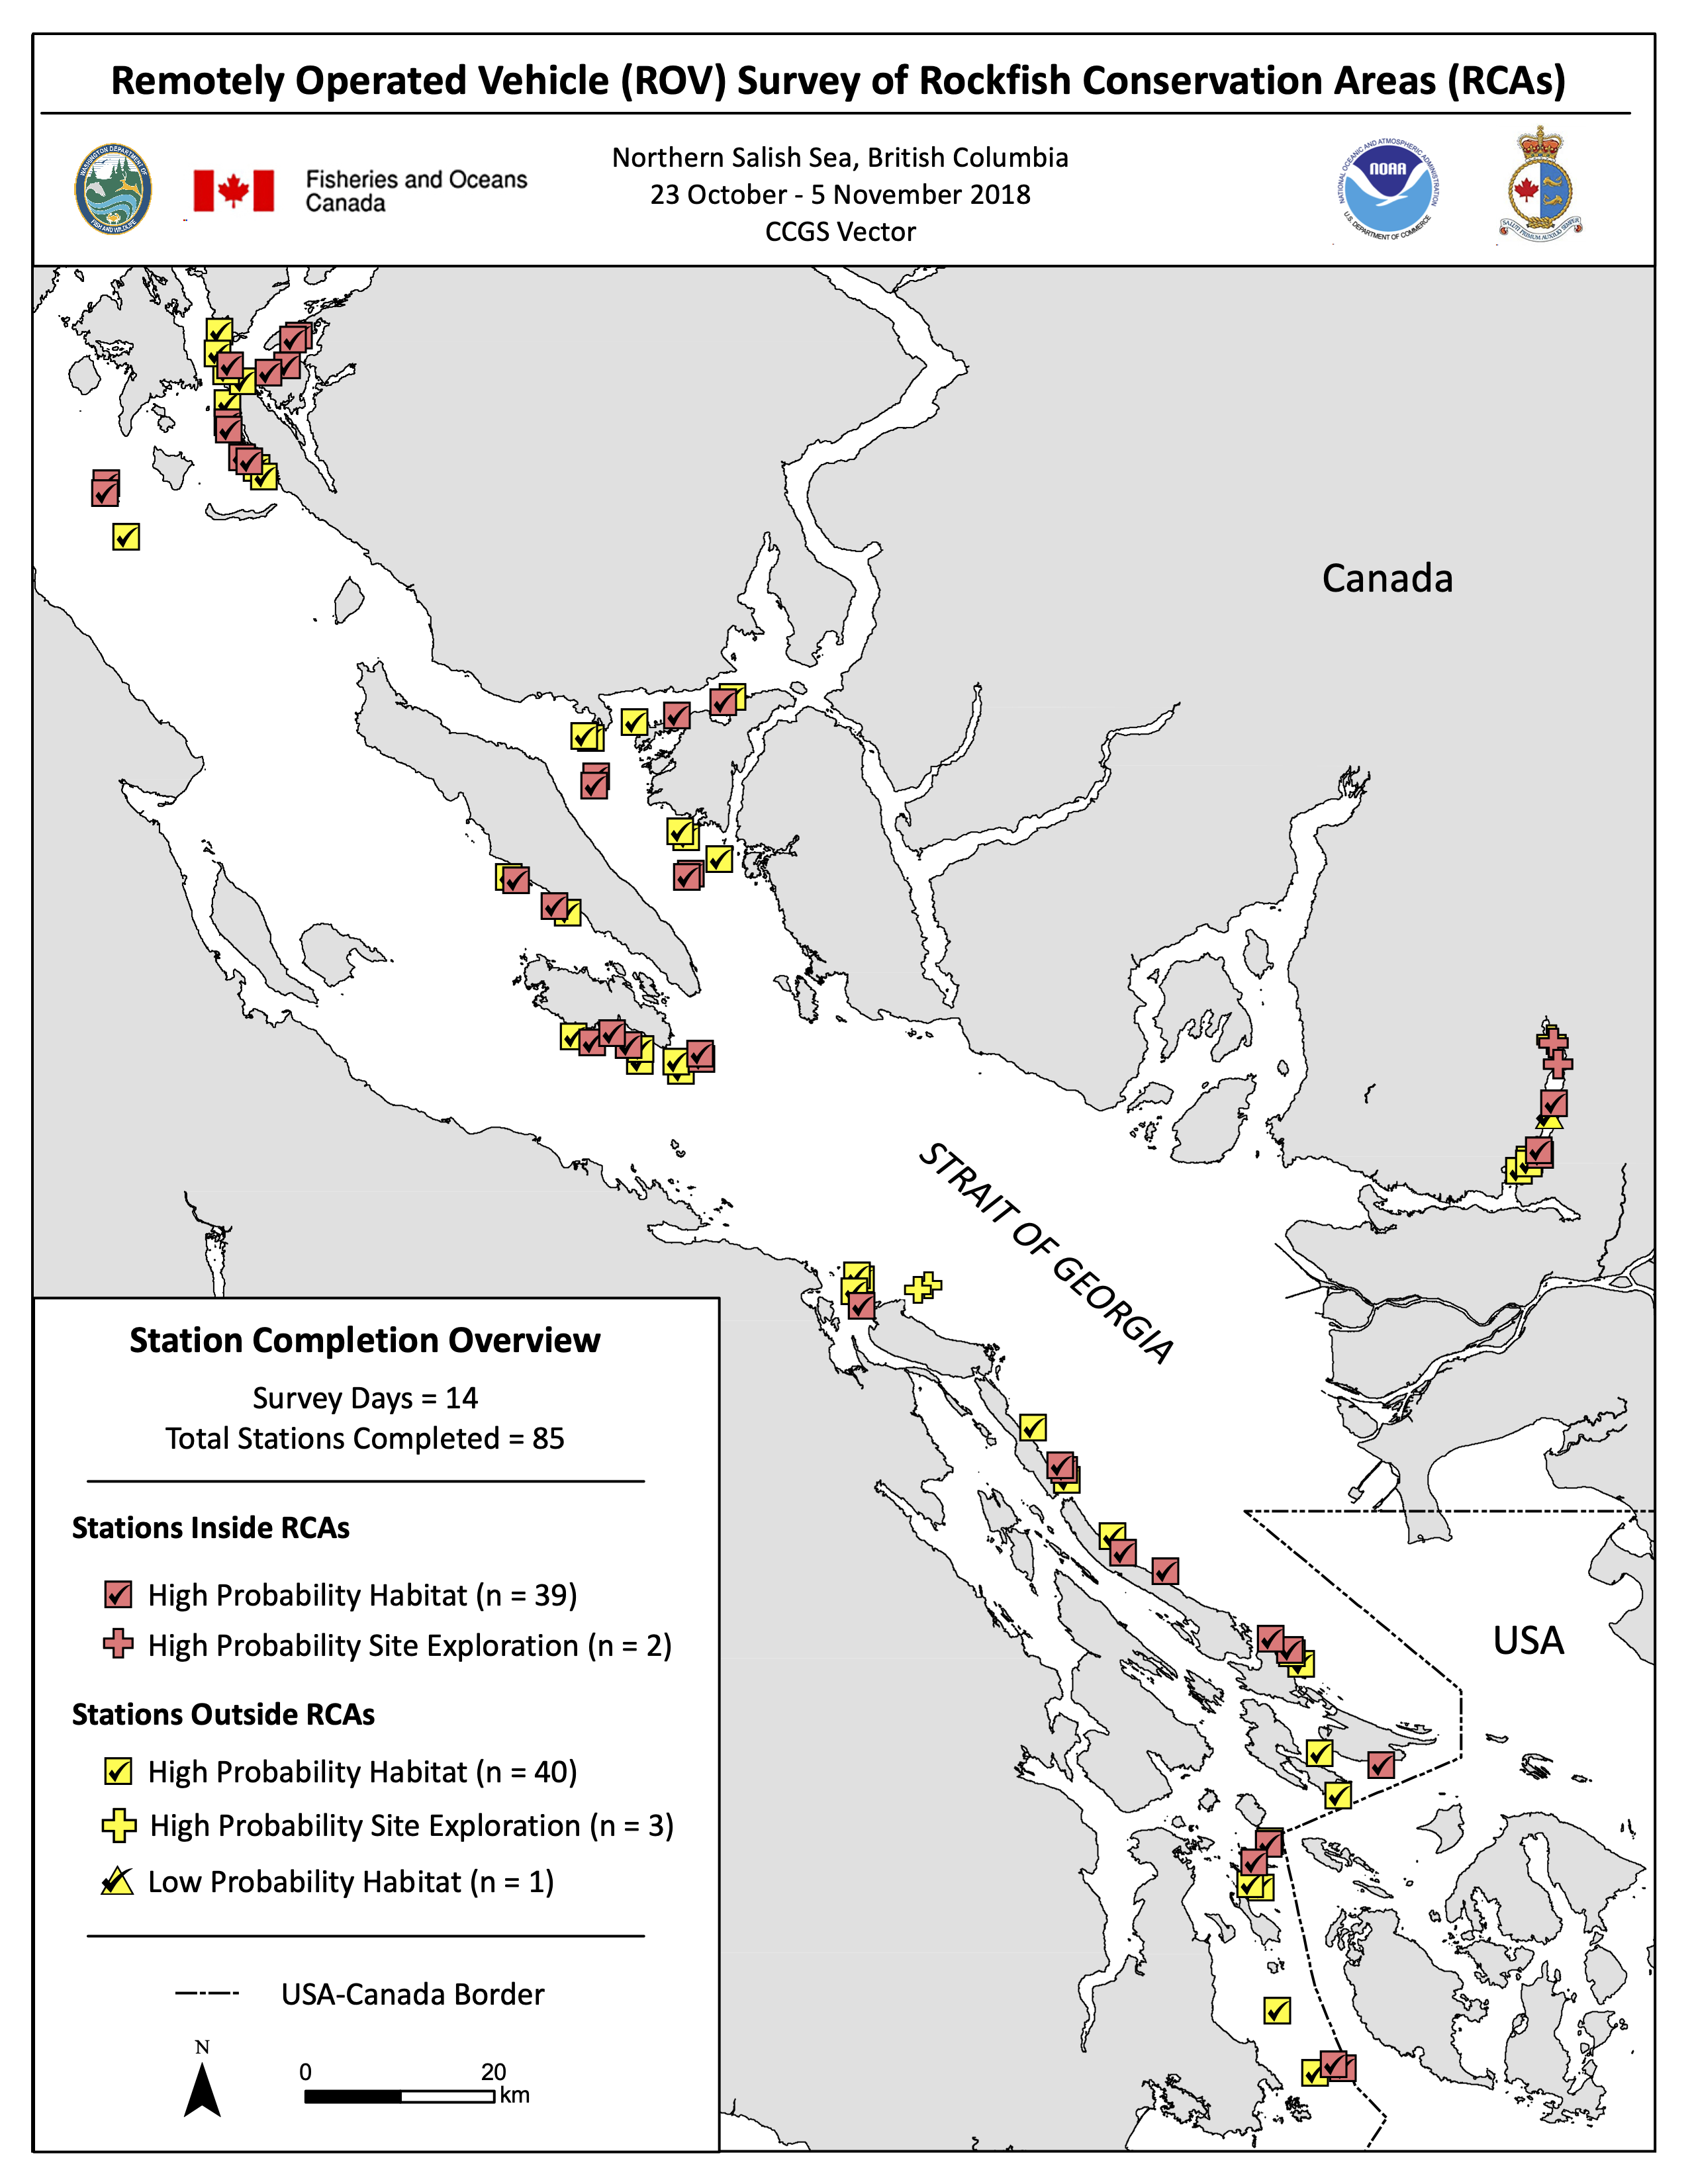
\includegraphics[width=1\textwidth,height=\textheight]{2018_vector_map.png}

\begin{itemize}
\tightlist
\item
  Maximum entropy (maxent) model
\item
  Survey strata: ``High'', ``Low''

  \begin{itemize}
  \tightlist
  \item
    High stratum

    \begin{itemize}
    \tightlist
    \item
      84 transects
    \item
      92,031 hectares
    \item
      198 yelloweye
    \end{itemize}
  \item
    Low stratum

    \begin{itemize}
    \tightlist
    \item
      1 transect
    \item
      816,993 hectares
    \item
      0 yelloweye
    \end{itemize}
  \end{itemize}
\item
  Population estimate: 1,613,716 (CV = 14.3\%)
\end{itemize}
\end{frame}

\end{document}
